\scanpage{223}
Il suffirait de construire $X$ projectif lisse sur $k$, tel que
$H^*(X_{\unsure{v|\nu}},\mathbf Z)$ et $H^*(X_{\unsure{w|\omega}},\mathbf Z)$
non isomorphes comme \uline{anneaux}.
On devrait mettre Serre à contribution.
\margin{Peut-on remplacer $\mathbf Z$ par $\mathbf R$ ??}
\figure{\begin{tikzpicture}\draw (0,0)--(2.5,0);\draw (.6,-.16)--(2,-.16);\end{tikzpicture}}

Soit $k$ un corps de nbs, $v_0$ une place de $k$, $M$ un motif sur $k$,
d’où $G_{Mv_0}=G_{v_0}$ grp algébrique \uline{défini sur} $\mathbf Z$.
Toute autre place \deleted{\unsure{de}} $v$ définit un fibré principal homogène
$P_v$ sous $G_{v_0}$,
\unsure{A} si on admet ce qui a été \deleted{dit}\inserted{conjecturé} plus haut,
\inserted{si $M$ est pris assez grand,}
\[
v\ne v'\Longrightarrow P_v\not\simeq P_{v'}.
\]
On peut aller plus loin et se demander si \deleted{\unsure{en}}
(pour $M$ assez grand) \uline{tt} fibré principal homogène $P$ sur $G_{v_0}$
provient d’une place $v$ \deleted{\unsure{complexe}}.
\figure{\begin{tikzpicture}\draw (0,0)--(.4,.6);\end{tikzpicture}}
\deleted{\unsure{les}} On \deleted{de} peut poser
\[
G_{Mv_{\unsure{0|a}}}(\mathbf Z)=\pi^1_M(k,v)
\]
\unsure{ces groupes} : \unsure{puis on est} \unsure{pour} \unsure{donner}
\unsure{nom} : groupes \uline{fondamentaux \inserted{(arithmétiques)} discrets}.
\margin{\figure{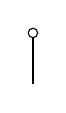
\begin{tikzpicture}\draw (0,0)--(0,.6);\draw (0,.65) circle (.06);\end{tikzpicture}}
Attention, la condition d’avoir un isomorphisme de foncteurs
$\xi(\unsure{N|M})\otimes_{\mathbf Z}\mathbf C\simeq M_\infty\otimes_k\mathbf C$,
satisfaisant aux conditions de compatibilité genre Riemann--Hodge,
risque d’être une condition \unsure{véritable sélection|véritable de sélection}....}
\figure{\begin{tikzpicture}\draw[->] (2,0)--(0,0);\end{tikzpicture}}
\margin{222}
